\documentclass[11pt]{article}
\usepackage{amsmath}
\usepackage{graphicx}
\usepackage{caption}
\usepackage{amssymb}
\usepackage{verbatim}
\usepackage{float}
\usepackage{hyperref}
\usepackage{listings}
\usepackage{euscript}
\setlength{\parindent}{0em}
\newcommand*{\field}[1]{\mathbb{#1}}%
\usepackage{amsthm}
\newtheorem{claim}{Claim}
\captionsetup{labelformat=empty}
\begin{document}



\begin{titlepage} % Suppresses displaying the page number on the title page and the subsequent page counts as page 1
	
	\center % Centre everything on the page
	
	\vspace*{8cm}
	\vfill\vfill
	\textsc{Mathemtical Tripos, Part 1B}\\
	\textsc{Computational project}
	\begin{center}
      {\huge\bfseries Random Binary Expansions}\\[0.4cm]
     \end{center}
	 % Title of your document
	
	\vfill
	
	
	
	
	%------------------------------------------------
	%	Date
	%------------------------------------------------
	\vspace*{\fill}
	\vfill\vfill\vfill % Position the date 3/4 down the remaining page
	
	{\large\today} % Date, change the \today to a set date if you want to be precise
	\vfill
	% Push the date up 1/4 of the remaining page	
\end{titlepage}


\section*{Question 1}
\subsection*{General description}
Identify the coin tosses are identically independent Bernoulli distributions with probability p, then the first program should be a function of three variables, namely n, N and p; A random sample is generated by the summation formula given in the problem description. 

The second half of the question is about approximating the distribution function by Monte Carlo simulation. I wrote a program to obtain the empirical distribution function for n=30, p=2/3 as requested, and chose a suitable N by error analysis. 

The program to find the EDF can be found at \textbf{Program 1} below

The program to generate a random sample can be found at \textbf{Program 2} below


\subsection*{Error analysis}
For this specific Monte Carlo simulation, the error can be quantified by the standard deviation of the empirical distribution function \^{F}, i.e.:
\begin{equation}
Random\ error =\sigma_{\hat{F}} =  \sqrt{F(1-F)/N}=O(N^{-1/2})
\end{equation}
It is reasonable to make the error approximately 0.01, and we should choose N=10000.

\subsection*{Graph}
The range of x was chosen as $\left[0,1\right]$
with interval 0.01. The empirical distribution function is 1 for $x\geq1$ and 0 for $x\leq1$.
\begin{figure}
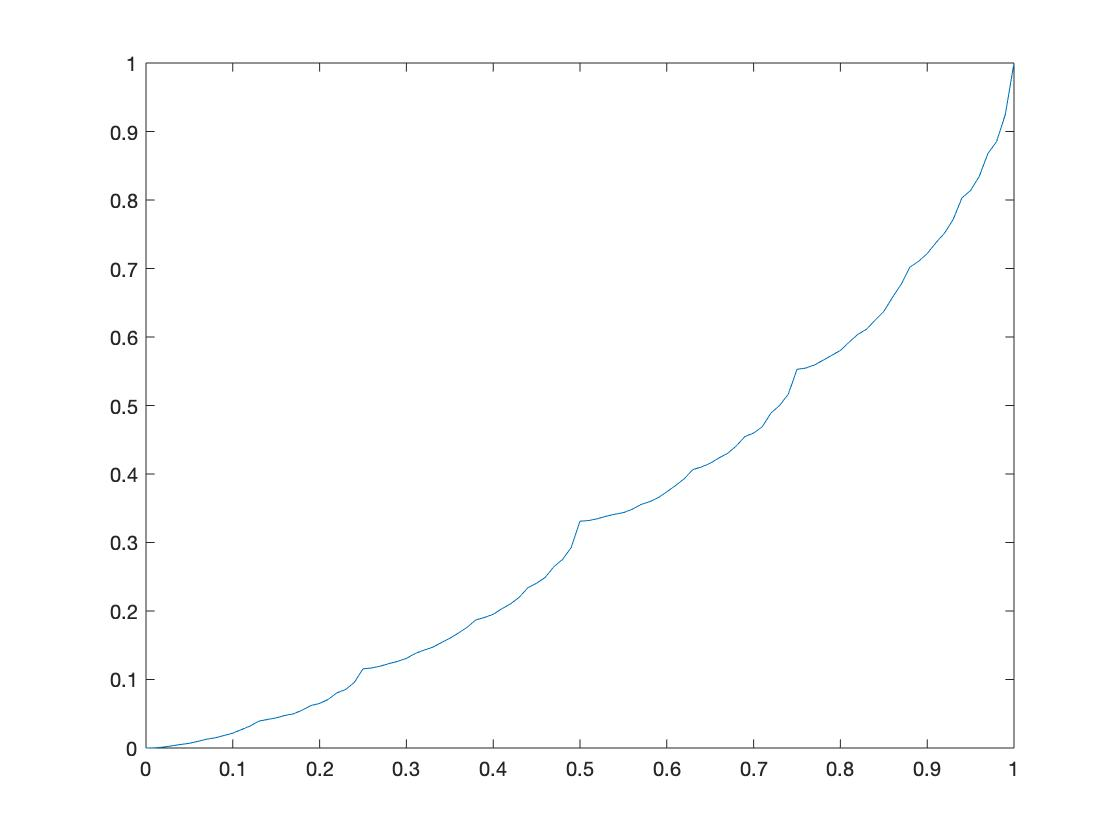
\includegraphics[width=13cm,height=8cm]{Q1}
\caption{\textbf{Figure 1.1:} Plot of $\hat{F} \ for\ x\in\left[0,1\right]$}
\end{figure}
\pagebreak
%\subsection*{Program 1: Empirical distribution function}
%\lstinputlisting{EDF.m}
%\subsection*{Program 2: Random Sample}
%\lstinputlisting{RandomSample.m}

\pagebreak
\section*{Question 2}
Without loss of generality, we shall write x as  
\begin{equation*}
x=\sum_{i=1}^{\infty}\frac{x_{i}}{2^{i}}
\end{equation*}
\subsection*{Calculation}
**In this and the following question, only consider binary expansion without an infinite tail of 1's.**\\
Any number smaller than or equal to x has the first n digits of binary expansion being a smaller number than x, so it is justified to consider only the first n digits .  
The relation: $x \sim y,\ x,y\in \left[0,1\right]$ if they have the same first n digits in binary expansion  is an equivalence relation, which is easy to verify. \\
\text{For} numbers less than or equal to x, there are exactly $$\sum_{i=1}^{n}2^{n}\frac{x_{i}}{2^{i}}=2^nx
$$ 
equivalence classes.  \\Consider digit-wise, let k denote the number of 1's in its first n digits, or u denote the number of 0's in its first n digits. The probability of obtaining such an equivalence class is $p^{k}q^{n-k}\ or\ p^{n-u}q^{u}.$
Hence the distribution function is as follows:\\
For x as given, 
$$F\left(x\right)=\sum_{i=1}^{2^{n}x}(q)^n(\frac{p}{q})^{k_{i}}$$
alternatively,
$$F\left(x\right)=\sum_{i=1}^{2^{n}x}(p)^n(\frac{q}{p})^{u_{i}}$$
Where $k_{i}$, $u_{i}$ are the numbers  of 1's and 0's in the first n digits of the ith equivalence class representation respectively.
\section*{Question 3}
\label{sec:Question 3}
The graph of F can be found at \textbf{Figure 2}.\\
The comparison graph is \textbf{Figure 3}.\\
The program is \textbf{Program 3}.\\\\
From \textbf{Figure 3}, it is obvious that the empirical distribution function gives an overestimate of the value of distribution function at each of x with a finite binary expansion. F is smoother than $\hat{F}$, and both functions are continuous and increasing by plot.\\ Quantitatively, observe that if the first digit of x is 0, i.e. $x<1$, then  $$F(\frac{x}{2})=qF(x)$$, otherwise $$F(\frac{x+1}{2})=pF(x)+q$$
Hence, 
\[F(x) = 
\begin{cases}
\ qF(2x)       & 0<x<0.5\\
\ pF(2x-1)+ q  & 0.5<x<1
\end{cases}\]
\subsection*{Time complexity}
The time complexity of the loop of Program 1 for general n, N is $\mathcal{O}\left(nN\right)$, and that of Program 3 is $\mathcal{O}\left(\sum_{i=1}^{2^{n}}y(i)\right) = \mathcal{O}\left(2^{2n-1}+2^{n-1}\right) = \mathcal{O}\left(2^{2n-1}\right)$. Therefore, for n large, program 3 takes much more time.
\begin{figure}
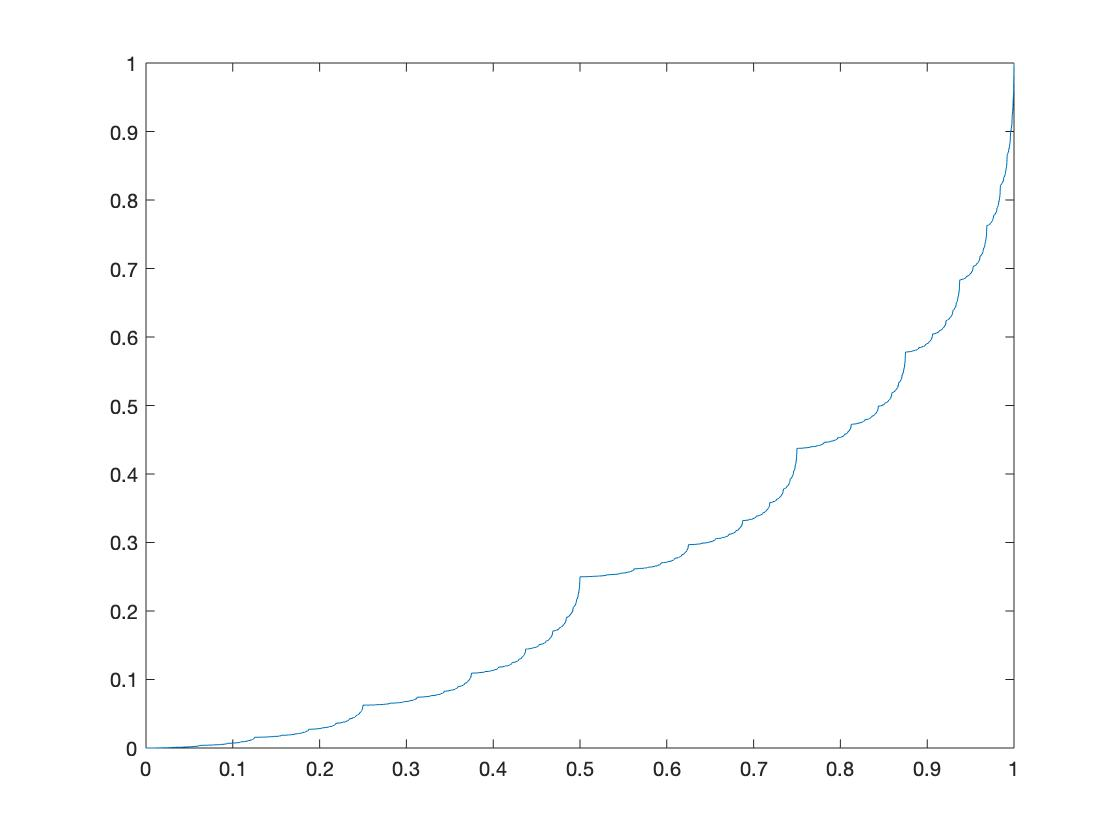
\includegraphics[width=13cm,height=8cm]{Q2}
\caption{\textbf{Figure 3.1:} Plot of $F \ for\ x\in\left[0,1\right]$}
\end{figure}

\pagebreak
%\subsection*{Program 3}
%\lstinputlisting{Q3.m}
%\pagebreak
\section*{Question 4}
\begin{claim}
If c $\in \left[0,1\right] $ has a finite binary expansion, then F is continuous at c.
\end{claim}
\begin{proof}
By 1A probability, for X an random variable,
\begin{equation*}
\mathbb{P}(\lbrace x=c\rbrace)=F_{X}(c)-F_{X}(c^{-})
\end{equation*}
and hence if $\mathbb{P}(\lbrace X=c \rbrace)=0$, X has a continuous distribution function.
For c with a finite binary expansion as in Question 3, $0<p,q<1$, 
\begin{equation*}
\mathbb{P}(\lbrace X=c \rbrace)=\lim_{k \to \infty}\prod_{i=1}^{n}(x_{i}p+(1-x_{i})q)^{x_{i}}q^{k}=0  
\end{equation*}
Therefore F is continuous at c.
\end{proof}
The plot suggests that F is continuous elsewhere.
\begin{claim}
F is continuous.
\end{claim}
\begin{proof}
Write $$x=\sum_{i=1}^{\infty}\frac{x_{i}}{2^{i}}$$, then
$$\mathbb{P}({X=c})=\prod_{i=1}^{\infty}(x_{i}p+(1-x_{i})q)^{x_{i}}=p^{m}q^{n}$$for some particular m,n.
If $0<p, q<1$, it is then enough to show that either m or n is infinite, which is true as x can have an infinite binary distribution anyway (e.g. for c can write $x=\sum_{i=1}^{\infty}\frac{x_{i}}{2^{i}}\ with\ x_{i} = 0\ for\  i > n$) . 
\end{proof}
\section*{Question 5}
The plots below suggest that F is right-differentiable at c, and the derivative is 0. The choice of delta is small enough compared with the value of c. In particular: The proportion of greatest value of delta is $\frac{2^{-11}}{2^{-1}+2^{-4}}\simeq0.1\% $ , which is suitable.

%\subsection*{Program 5}
%\lstinputlisting{Q5.m}
%\textbf{Input values:}
%\lstinputlisting{delta.m}
\begin{figure*}[h]
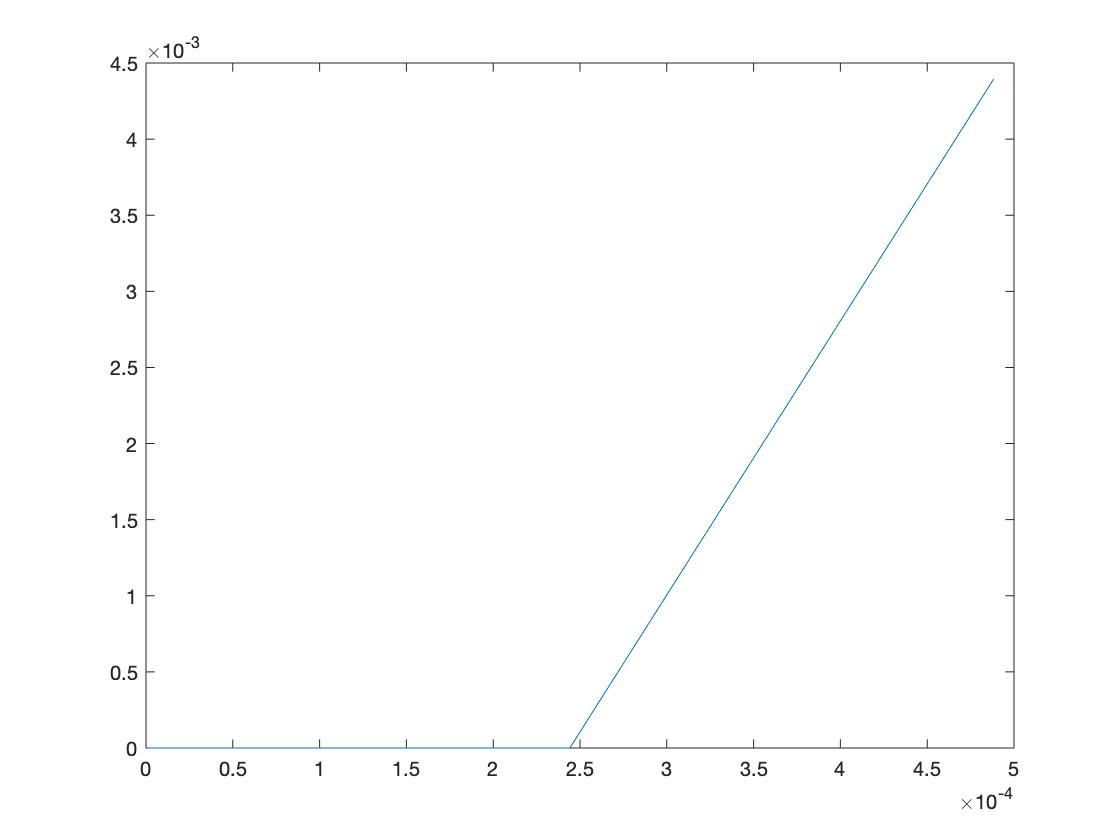
\includegraphics[width=13cm,height=8cm]{Q5(1).jpg}
\caption{\textbf{Figure 5.1:} Output of Q5(x, 3/4, 11, 9/16) , note that it vanishes at x close to 0. }
\end{figure*}
\begin{figure*}
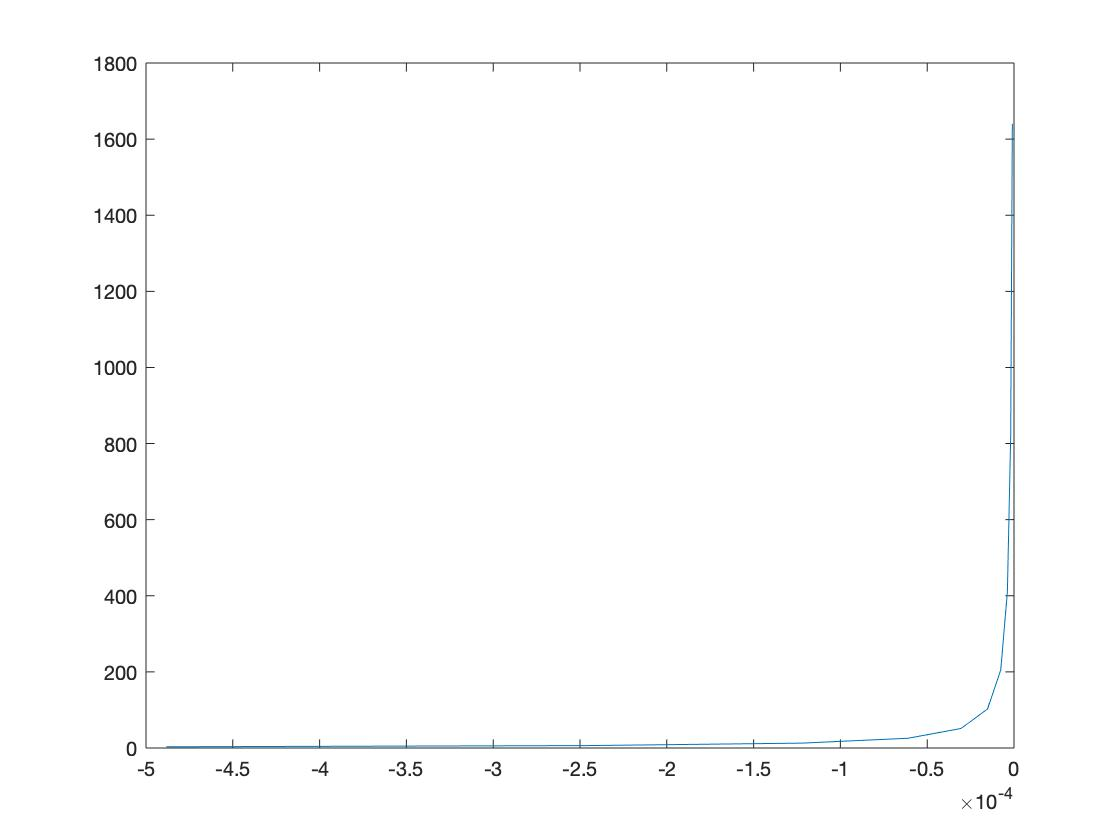
\includegraphics[width=13cm,height=8cm]{Q5(2).jpg}
\caption{\textbf{Figure 5.2:} Output of Q5(y, 3/4, 11, 9/16)}
\end{figure*}
\pagebreak

\section*{Question 6}
\newtheorem{conjecture}{Conjecture}
\begin{conjecture}
F is right-differentiable at an arbitrary point c with a finite binary expansion.
\end{conjecture}
\begin{proof} 


**$k_{i}$, $u_{i}$ used below are as in Question 2.**
\\If c has a finite binary expansion as in Question 3, then c=$\frac{m}{2^n}$ for some $ m\in \mathbb{N}$.
Then$$\lim_{l \to \infty}\frac{F(c+2^{-(n+l)})-F(c)}{2^{-(n+l)}}=\lim_{l \to \infty}\frac{F(\frac{2^lm+1}{2^{n+l}})-F(\frac{2^{l}m}{2^{n+l}})}{2^{-(n+l)}}=\lim_{l \to \infty} (2q)^{n+l} (\frac{p}{q})^{k_{2^lm+1}}$$
where $ k_{2^lm+1}$ is a constant for a fixed c.
Hence, the limit exists and is finite when $q<\frac{1}{2}$.
Similarly, by approaching from the left,
$$\lim_{l \to \infty}\frac{F(\frac{2^lm-1}{2^{n+l}})-F(\frac{2^{l}m}{2^{n+l}})}{-2^{-(n+l)}}=\lim_{l \to \infty} (2p)^{n+l} (\frac{q}{p})^{u_{2^lm}}$$
where $u_{2^{l}m}$ is smaller than n for a fixed c, as the binary expansion of the $2^{l}m$ th number is of value $m{-}\frac{1}{2^{n+l}}$ which has at least \textit{l} 1's out of the n+\textit{l} digits.
Hence the limit exists and is finite when $p<\frac{1}{2}$. 
Therefore, F is left-differentiable when $p<\frac{1}{2}$, and right-differentiable when $p>\frac{1}{2}$.
At $p = \frac{1}{2}$, by the distribution function, it is a straight line joining 0 \& 1.
\end{proof}
\subsection*{Graphic support}
At $c=\frac{10}{16}$, with p=3/7, 
\textbf{Input values:} 
\lstinputlisting{deltacopy.m}
The following graphs \textbf{6.1}, \textbf{6.2} and \textbf{6.3} support the conjecture.
\begin{figure}[H]
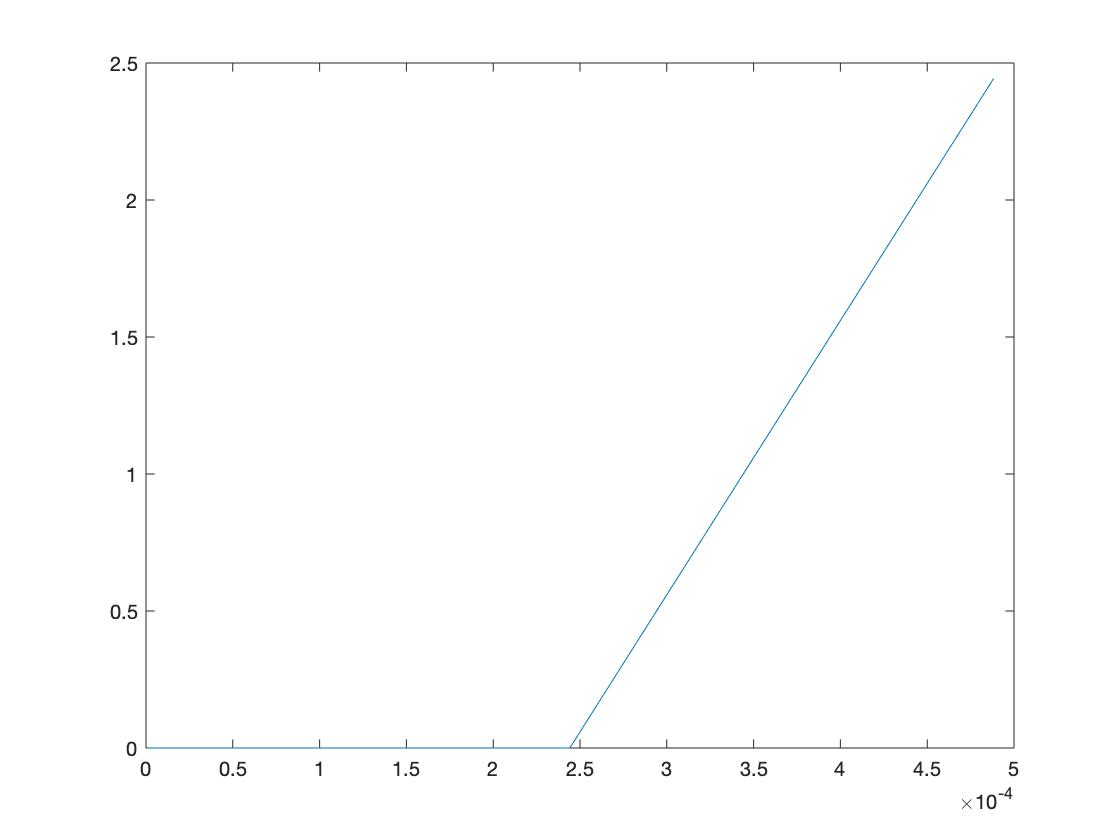
\includegraphics[width=13cm,height=8cm]{Q6(1).jpg}
\caption{\textbf{Figure 6.1:} Output of Q5 (x, 3/7, 11, 10/16)}
\end{figure}
\begin{figure}
\includegraphics[width=13cm, height=8cm]{Q6(2).jpg}
\caption{\textbf{Figure 6.2:} Output of Q5 (y, 3/7, 11, 10/16)}
\end{figure}
\begin{figure}
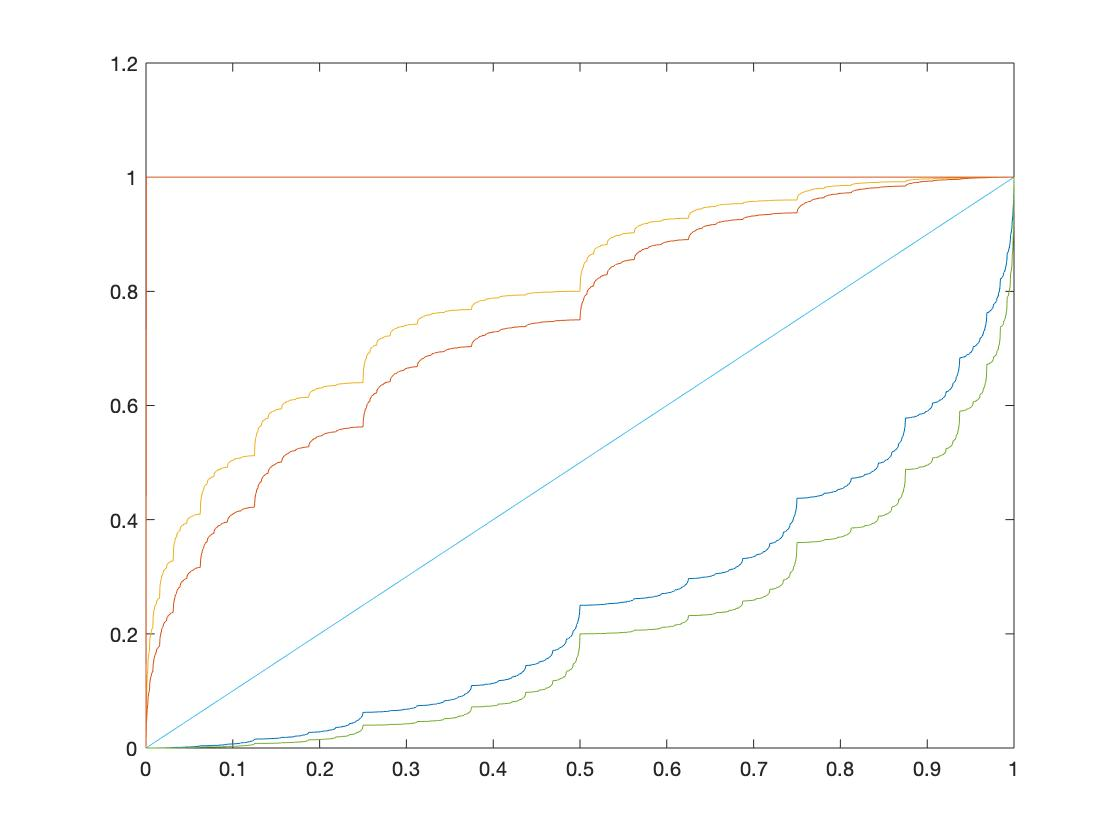
\includegraphics[width=13cm, height=8cm]{Q6(3).jpg}
\caption{\textbf{Figure 6.3:} Output of Q3 with p=1,0,1/2,1/4,1/5,3/4,4/5}
\end{figure}
\subsection*{Program 1: Empirical distribution function}
\lstinputlisting{EDF.m}
\subsection*{Program 2: Random Sample}
\lstinputlisting{RandomSample.m}
\subsection*{Program 3: Distribution Function}
\lstinputlisting{Q3.m}
\subsection*{Program 4: Question 5}
\lstinputlisting{Q5.m}
\textbf{Input values:}
\lstinputlisting{delta.m}











\end{document}

